\chapter{Modules systèmes}
\label{ch:module_systems}





% Définition sommaire d'une bibliothèque de code
Une bibliothèque de code est le regroupement de plusieurs types de données, des
entiers, des nombres à virgule flottant, des chaînes de caractères, des
fonctions et des données composites. L'ensemble de ces données constitue les
fonctionnalités de la bibliothèque.  Les fonctionnalités d'une bibliothèque
peut être copié dans l'exécutable (bibliothèque statique), cela facilité la
distribution du binaire puisque que ses dépendances sont inclus dans
l'exécutable.  Les fonctionnalités d'une bibliothèque peuvent aussi être chargé
à l'exécution (bibliothèque partagés), cela permet de partagé des routine
commune entre plusieurs processus (programme en exécution). Les données de la
bibliothèque, par contre, ne sont partagé, chaque processus réfère à sa propre
version des données.  Le format d'une bibliothèque de code varie d'un langage à
l'autre et aussi d'un système d'exploitation à un autre. Les langages
interprétés utilisent plus souvent le code source directement ou une
représentation intermédiaire comme format pour les bibliothèques de code.  Pour
les langages compilés, c'est le format natif correspondant au système
d'exploitation qui est le plus souvent utilisé. Le système d'exploitation Linux
utilise le format ELF (\textit{Extensible Linking Format}), Microsoft Window
utilise le format PE (\textit{Portable Executable}) et MacOSX utilise le format
Mach-O (\textit{Mach object}) pour les exécutables et les bibliothèques.
% XXX: bytecodes aussi pour les langage compilé.

%Les langages
%de programmation interprétés fournisse leurs bibliothèques directement
%en code source. Dans cette catégorie, il y a Ruby, Python, Perl, Lua et
%Scheme -- dont le code des bibliothèques est écrit et frounit dans le
%langage respectif. Les langages compilés -- comme C, C++, C\# et Java --
%utilisent plutôt des formats binaires destiné, soit à une machine virtuelle
%(e.g. la \textit{Java Virtual Machine} JVM ou un architecture
%physique (e.g. i686, x86\_64, ARM). Les bibliothèques natives peuvent
%être utilisé


\section{Édition de liens dynamique}

Une application qui utilise une bibliothèque partagés ne contient pas le code
de la bibliothèque, mais plutôt le nom des fonctionnalités utilisés.  La
routine qui permet de récupérer la fonctionnalité à partir du nom est la
résolution qui est effectué par le \textit{dynamic loader}.  Lorsqu'un
programme lié dynamiquement à plusieurs bibliothèques partagés exécute du code
externe \verb|foo|, un routine de résolution est démarré pour déterminé quelle
bibliothèque lié au fournit la fonctionnalité \verb|foo|.

%% Bibiothèque dynamique native.
Par exemple, sous Linux l'utilitaire <<yes>>, qui est écrit en C,
est lié aux bibliothèques systèmes suivantes:
\begin{verbatim}
  linux-vdso.so.1 (0x00007ffeef7f9000)
  libc.so.6 => /usr/lib/libc.so.6 (0x00007ff68161c000)
  /lib64/ld-linux-x86-64.so.2 => ...
\end{verbatim}
La bibliothèque \textit{libc.so.6} contient la plupart des fonctions
standards du système sous Linux dont les fonctionnalités sont résolut
à l'exécution.
% Le but d'une bibliothèque est la réutilisation de code.
Dans le contexte d'un exécutable natif, le chargement des bibliothèques
s'effectue au début de l'application, avant l'exécution de la fonction principale
souvent nommé \textbf{main}. Plusieurs bibliothèques peuvent coexister simultanément au
sein d'un même processus sans que l'exécution du programme en soit affecté.

La résolution des fonctionnalité de ces bibliothèques sont effectué par un programme adapté
le \textit{program interpreter} du système qui correspond à \textit{/lib64/ld-linux-x86-64.so.2}.
Il est possible de forcer la résolution d'une fonctionnalité d'une bibliothèque
de façon manuel. Ce genre d'interaction est possible sur
les trois principales plateformes utilisées sur le marché (Windows, MacOSX et Linux).

%% TODO: continue here FIXME
Sur Linux, l'API qui permet d'interagir avec les bibliothèques partagés provient de \textit{libdl.so}.
Elle contient les fonctions \textit{dlopen}, \textit{dlsym}, \textit{dlerror} et \textit{dlclose} pour gérer
des bibliothèques de code supplémentaire chargé manuellement à l'exécution.  Pour charger la fonction
\textit{foo}, qui ne prend pas d'argument et ne retourne rien de la bibliothèque \textit{libFoo.so} en C,
il faut exécuter les deux appels suivant:
\begin{center}
  \begin{figure}[ht]
\begin{lstlisting}[language=C,frame=single]
  ...
  void *handle = dlopen("./libFoo.so", RTLD_LAZY);
  void (*foo)() = dlsym(handle, "foo");
  ...
\end{lstlisting}
\caption{Chargement dynamique de la bibliothèque \textit{libFoo.so} et
résolution de la fonction \textit{foo} sans gestion d'erreur sous Linux}
  \end{figure}
\end{center}
L'équivalent des bibliothèques partagés sous Window sont les DLLs, ils peuvent être chargé de façon similaire dans un
programme en utilisant les fonctions \textit{LoadLibrary}, \textit{LoadLibraryEx} et \textit{GetProcAddress}. Ils
fonctionne de la même façon que leur équivalent Linux. Pour MacOSX, il faut passer par les routines:
\begin{itemize}
    \item \textit{NSCreateObjectFileImageFromFile}
    \item \textit{NSLinkModule}
    \item \textit{NSLookupSymbolInModule}
    \item \textit{NSAddressOfSymbol}
\end{itemize}

La majorité des langages interprétés permettent l'importation de bibliothèque de code natif, via un interface
nommé \textit{foreign function interface}.
Prenons comme exemple les langage Python, Ruby, Lua et Scheme. Python possède le module ctypes
qui permet de chargé des bibliothèques natives dynamique, Ruby possède le module ffi.
%Ces modules ne font qu'encapsuler les fonction de chargement de bibliotheques native pour qu'il puisse être invoqué
%dans le langage cible.

% Bibliothèque Lua en C
% - La bibliothèque doit avoir le même nom que celui utilisé par le \textit{import}.

Certains langages ont même un mécanisme pour charger des bibliothèques natives s'ils ont été conçus spécialement.
Dans le langage de programmation Lua, il est possible en Lua de chargé directement
une bibliothèque dynamique si elle contient une fonction principale \textbf{luaopen\_\textit{libname}}
où \textit{libname} est le nom de la bibliothèque.

Gambit Scheme utilise un mécanisme équivalent. Il permet le chargement de ces modules qui ont été compilé
en bibliothèque partagé (DLL) avec la fonction \textit{(\textbf{load} "libname")}. Le chargements de la
bibliothèque ressemble à celui de Lua.

%% Python
%\begin{figure}[ht]
%\begin{lstlisting}[language=python,frame=single]
%# From https://docs.python.org/2/library/ctypes.html
%from ctypes import *
%# Chargement d'une bibliotheque native.
%lib = cdll.LoadLibrary("./libFoo.so")
%# Appel de la fonction foo.
%lib.foo()
%\end{lstlisting}
%\caption{Code d'importation de la fonction \textbf{foo} de la bibliothèque \textit{libFoo.so} en Python}
%\end{figure}

\begin{center}
% Ruby
\begin{figure}[ht]
\begin{lstlisting}[language=ruby,frame=single]
require 'ffi'
# Chargement d'une bibliotheque native.
module LibFoo
    extend FFI::Library
    ffi_lib './libFoo.so'
    attach_function :foo, [], :void
end
# Appel de la fonction foo.
LibFoo.foo
\end{lstlisting}
\caption{Code d'importation de la fonction \textbf{foo} de la bibliothèque \textit{libFoo.so} en Ruby}
\end{figure}
\end{center}

La résolution des fonctionnalités effectué par le \textit{dynamic linker} utilise un ordre de recherche
définit. Cet ordre de recherche inclut l'exécutable courant, les dépendances de l'exécutable, la bibliothèque
passé à \textit{dlsym}. La résolution d'une fonctionnalité par \textit{dlsym} qui n'engendre pas la résolution
d'un autre fonctionnalité externe n'utilise pas le programme principale dans l'ordre de recherche qui alors
commence par la bibliothèque passé à \verb|dlsym| suivit de ses dépendances. Les résolution de fonctionnalité
provenant d'appels indirecte au \textit{dynamic linker} inclut le programme principal et ses dépendances avant
la bibliothèque passé à \verb|dlsym|.

\begin{center}
    \begin{figure}[ht]
        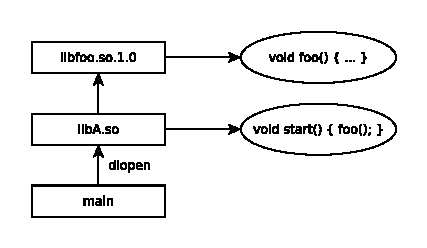
\includegraphics{figures/libdeps-ex1.pdf}
        \caption{Un exemple de dépendance de bibliothèques au sein d'un application simple fictive.
            La bibliothèque \textit{libA.so} est chargé dans l'application \texttt{main} via
            les appels au procédure \textit{dlopen} et \textit{dlsym}. Le fonctionnalités utilisés
            dans l'exemple sont marqué par un ellipse.
        }
        \label{fig:deps-ex1}
    \end{figure}
\end{center}

Dans la situation situation présenté dans la figure-\ref{fig:deps-ex1}, quels sont les étapes inclut
dans l'exécution de ce programme qui ne fait qu'appeler la fonctionnalité \texttt{start} de la
bibliothèque \textit{libA.so}. La fonctionnalité \texttt{start} est résolu de façon direct par
un appel à \verb|dlsym(libA, "start")|, qui commence la recherche de la procédure \texttt{start} dans
la bibliothèque spécifier dans \texttt{dlsym}. Le programme, une fois la procédure trouvé, l'exécute.
L'appel à une procédure non résolue (e.g.\ la procédure \texttt{foo} invoqué dans \texttt{start})
déclenche une procédure automatique de résolution des fonctionnalités. Cette procédure de résolution
commence sa recherche à partir de l'exécutable, puis itère la liste des dépendances directe. Si la
fonctionnalité n'est pas encore trouvé, la recherche continuera à partir de la bibliothèque passé à
\texttt{dlsym}.

% Stub

% TODO: exemple de résolution direct
Connaissant l'ordre de recherche du \textit{dynamic linker}, il est facile de construire un application avec des bibliothèques
qui cause un masquage de fonctionnalité. Deux possibilité facilement exploitable, faire que l'exécutable main fournisse
directement la fonctionnalité à masquer, ou avoir une des dépendances de l'exécutable contenant cette fonctionnalité. La figure-\ref{fig:deps-ex2}
en est l'exemple qui utilise la seconde méthode. La première consisterait à transformer l'exécutable main est bibliothèque
exécutable qui ne pourrait pas être supporté sur certaine plateforme. Sous Linux, il est possible de créer une bibliothèque qui
exécutable en passant le paramètre \texttt{-rdynamic} à \textit{gcc} lors de la construction.

\begin{center}
    \begin{figure}[ht]
        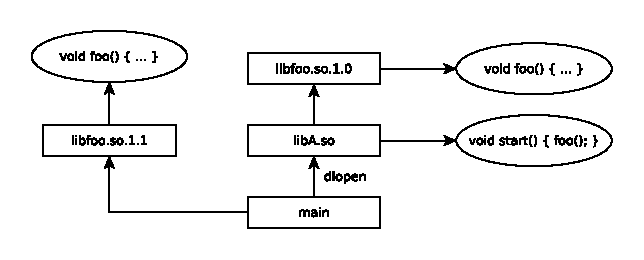
\includegraphics{figures/libdeps-ex2.pdf}
        \caption{Exemple de dépendance dans un application cause le masquage de la fonctionnalité \texttt{foo}
        de la bibliothèque \textit{libfoo.so.1.0} par la bibliothèque \textit{libfoo.so.1.1}}
        \label{fig:deps-ex2}
    \end{figure}
\end{center}
%% BEGIN
% D'autre langage compilé comme C/C++
% ne le permette pas directement, la liste des bibliothèques de code utilisé par un
% programme est déterminée lors de la création du fichier binaire, qui peut être
% soit un exécutable où une bibliothèque.
%% END


% TODO: pourquoi est-ce utile?
% XXX: structure pas final.
% - Les bibliothèques coexistent dans les application de tous les jours.
Analyser les interactions entre des bibliothèques au sein d'un même programme permet de
mieux comprendre quels sont les circonstance qui peuvent conduire à des comportements
non désirés, par exemple le masquage démontré dans la figure-\ref{fig:deps-ex2}.
Cela permet aussi d'établir les conditions qui inhibe ces comportements non désirés.


